\documentclass[10pt,conference,compsocconf]{IEEEtran}

\usepackage{hyperref}
\usepackage{graphicx}
\usepackage{booktabs}
\usepackage{amsmath}

\begin{document}
\title{Predicting Coronary Heart Disease from Lifestyle Surveys\\with Regularised Logistic Regression}

\author{
  Moncef Hafiz, Melek Fendri, Rayen Anane\\
  \textit{CS-433 Machine Learning, EPFL, Switzerland}
}

\maketitle

\begin{abstract}
We predict whether a respondent of the 2015 BRFSS telephone survey has been
diagnosed with coronary heart disease (MICHD) from 321 self-reported answers.
Using only NumPy, we build a feature pipeline that respects the survey's
coding conventions and train an $L_2$-regularised logistic regression with
Newton's method. Tuning the decision threshold for F1 is by far the most
important design choice (F1 0.237$\,\to\,$0.431); feature engineering adds
+0.016 over raw features, and logistic regression beats the least-squares
baselines by about 0.01 F1. Our final model reaches a 5-fold cross-validated
F1 of $0.431\pm0.006$ (AUC 0.861).
\end{abstract}

\section{Introduction}
The dataset contains $N=328{,}135$ training and $109{,}379$ test respondents
described by $D=321$ raw survey variables; only $8.8\%$ of respondents are
positive. The competition metric is the F1 score of the positive class. We
compare the six methods implemented in \texttt{implementations.py} with a
Newton-trained logistic regression and quantify the contribution of each
preprocessing step with an ablation study.

\section{Data and Preprocessing}
\label{sec:prep}
\textbf{Exploration.} Variables are of three kinds: (i) categorical answers
coded $1,2,\dots$ in which 7 means ``don't know'' and 9 ``refused'';
(ii) counts or measurements with \emph{special codes} (e.g.\ in
\texttt{PHYSHLTH}, 88 means ``zero days'' and 77/99 are non-answers);
(iii) survey-administration fields (interview date, sequence number,
sampling weights). 99 columns are more than $90\%$ missing because they
belong to optional state modules.

\textbf{Pipeline.} All statistics are fit on the training data only (and
re-fit inside every CV fold).
(1)~We drop 31 administration/weight columns and 18 raw answers with a
mixed unit encoding (e.g.\ \texttt{FRUIT1}, where $1xx$ = per day, $2xx$ =
per week) for which the CDC provides a cleaned computed variable, as well as
columns with $>90\%$ missing values.
(2)~Columns with $\le 15$ distinct values (and \texttt{\_STATE}) are
\emph{one-hot encoded}, with a separate level for missing values; levels
seen fewer than 50 times are dropped. Codes 7/9 thus become indicators
instead of being read as large numbers.
(3)~For the 42 continuous columns we \emph{decode special codes}
(88$\to$0; 77, 99, 900, 99900$\to$missing), apply $\log(1+x)$ to
non-negative columns with skewness $>2$, \emph{clip} to the 1st--99th
percentiles, impute the median, add a \emph{missing indicator} and
standardise. The result has 814 features plus a bias.

\section{Models and Evaluation}
\textbf{Baselines.} Least squares, ridge regression (normal equations, on
targets $y\in\{0,1\}$, prediction $x^\top w>t$) and regularised logistic
regression trained by gradient descent (300 steps, $\gamma=1/L$ with $L$
the Lipschitz constant of the gradient, estimated by power iteration).

\textbf{Final model.} We minimise the logistic loss plus
$\lambda\|w_{1:}\|^2$ (bias unpenalised) with Newton's method: each step
solves $(X^\top S X/N + 2\lambda I)\,\Delta w=\nabla$ with
$S=\mathrm{diag}(p_i(1-p_i))$. It converges in 8 steps ($\sim$1\,min)
where gradient descent is still far from the optimum after 300 steps, which
makes cross-validated model selection affordable.

\textbf{Threshold.} With $8.8\%$ positives, the Bayes threshold $p=0.5$
maximises accuracy, not F1. We choose the threshold $t$ that maximises F1 on
the training folds by sorting the scores (exact search) and apply it to the
held-out fold. On the full data $t$ corresponds to $p=0.20$.

\textbf{Protocol.} Stratified 5-fold CV (seed 0) for every number below; we
report the mean $\pm$ std over folds of F1, accuracy and ROC-AUC.

\section{Results}

\begin{table}[t]
\centering
\caption{5-fold CV results. All models use a tuned threshold unless stated.}
\label{tab:results}
\footnotesize\setlength{\tabcolsep}{4pt}
\begin{tabular}{@{}lccc@{}}
\toprule
Model / variant & F1 & Acc. & AUC \\
\midrule
\multicolumn{4}{@{}l}{\emph{Baselines (implementations.py), full features}}\\
Least squares & \multicolumn{3}{c}{$X^\top X$ singular} \\
Ridge, $\lambda=10^{-4}$ & $.422\pm.006$ & .872 & .854 \\
Reg.\ logistic, GD 300 it. & $.406\pm.003$ & .860 & .848 \\
Ridge, raw features & $.410\pm.005$ & .871 & .844 \\
\midrule
\textbf{Newton logistic, $\lambda=10^{-4}$ (final)} & $\mathbf{.431\pm.006}$ & .871 & \textbf{.861} \\
\midrule
\multicolumn{4}{@{}l}{\emph{Ablation of the final model}}\\
-- threshold tuning ($p>0.5$) & $.237\pm.005$ & .915 & .861 \\
-- thr.\ tuning, + class-balanced weights & $.378\pm.003$ & .767 & .861 \\
+ class-balanced weights & $.429\pm.007$ & .872 & .861 \\
-- one-hot (raw codes as numbers) & $.426\pm.006$ & .873 & .859 \\
-- special-code decoding & $.430\pm.007$ & .873 & .861 \\
-- log transform and clipping & $.430\pm.006$ & .871 & .861 \\
-- missing indicators & $.431\pm.006$ & .873 & .861 \\
+ administration/weight columns & $.430\pm.007$ & .873 & .861 \\
+ squared continuous features & $.431\pm.006$ & .873 & .861 \\
Raw features only (mean-imputed) & $.415\pm.005$ & .868 & .851 \\
\bottomrule
\end{tabular}
\end{table}

\begin{figure*}[t]
\centering
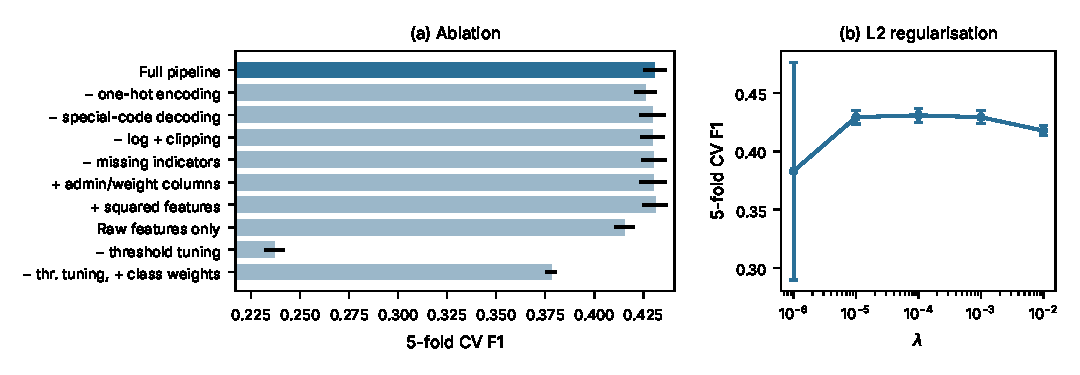
\includegraphics[width=0.9\textwidth]{../figures/ablation.pdf}
\caption{(a) 5-fold CV F1 of the ablation variants (bars: std over folds).
(b) F1 versus the $L_2$ penalty $\lambda$ of the Newton logistic regression.}
\label{fig:ablation}
\end{figure*}

Table~\ref{tab:results} and Fig.~\ref{fig:ablation} summarise the
experiments.

\textbf{Threshold is the dominant factor.} Predicting $p>0.5$ yields the
best accuracy (0.915) but an F1 of only 0.237, because few respondents reach
$p>0.5$. Re-weighting the classes recovers part of the gap (0.378), but
tuning the threshold directly gives 0.431; once the threshold is tuned,
class weights bring nothing (0.429): the AUC is unchanged, so the ranking
of respondents is the same and only the operating point moves.

\textbf{Model.} Logistic regression outperforms ridge regression by +0.009
F1 and +0.007 AUC on identical features: the squared loss penalises
confident correct predictions and is ill-suited to a rare binary target.
Plain least squares fails outright: every one-hot block (including its
missing level) sums to the bias column, so $X^\top X$ is singular. The same
collinearity explains Fig.~\ref{fig:ablation}(b): for $\lambda=10^{-6}$ the
Hessian is nearly singular and the undamped Newton iteration becomes
unstable on some folds (F1 $0.38\pm0.09$), whereas $\lambda\in[10^{-5},
10^{-3}]$ gives a flat optimum; $\lambda=10^{-2}$ underfits (0.418).
Gradient descent with the same objective reaches only 0.406 after 300 steps,
showing that the optimiser, not the model, limits the GD baseline.

\textbf{Feature engineering.} The full pipeline improves F1 by +0.016 and
AUC by +0.010 over raw mean-imputed features, for both ridge and logistic
regression. One-hot encoding is the most useful single step ($-0.005$ when
removed). Removing any other single step costs at most 0.001, below the
fold-to-fold std: the steps are partly redundant (e.g.\ decoding is only
needed for 13 continuous columns since one-hot already isolates codes 7/9 in
categorical ones). Squared features bring $+0.0002$ for 42 extra columns
and were not kept. Keeping the administration columns does not help either,
which is reassuring: the model does not exploit artefacts of the survey
process.

\textbf{Interpretation.} The largest coefficients correspond to a previous
stroke, male sex, poor self-rated general health, COPD, kidney disease, age
and estimated cardiorespiratory fitness (\texttt{MAXVO2\_}, negative)
--- all known cardiovascular risk factors.

\section{Conclusion}
A carefully regularised linear model, trained with a second-order optimiser
and evaluated with the metric's own decision rule, reaches a CV F1 of 0.431.
Choosing the operating point mattered far more than any single
preprocessing step; the remaining gap is likely due to the linear decision
boundary, which non-linear models (Project 2) could address. Our submission
is reproduced by \texttt{run.py}; every number above is produced by
\texttt{experiments.py}.

\end{document}
